%\section{結果}
\section{得られた結果}
\subsection{アルゴリズムの開発・改良と一般のコンピュータ1台での実行}
\subsubsection{利用した一般のコンピュータの性能}
今回計算に用いた一般のコンピュータの性能を表\ref{tb:normalpc-perf}に示す。

\begin{table}[htb]
	\begin{center}
	\begin{tabular}{|l|l|}
\hline \hline
\multicolumn{1}{|c|}{項目} & \multicolumn{1}{|c|}{仕様} \\
\hline \hline
CPU & Intel Pentium 4 \ 3.20GHz \\
CPUコア数 & 2 cores \\
CPUピーク性能 & 6.40GFLOPS \\
CPUメモリ & 3GB \\
OS & Linux 3.2.46 \\
コンパイラ & GCC 4.7.2 \\
\hline
	\end{tabular}
	\end{center}
	\caption{一般のコンピュータの性能概要}
	\label{tb:normalpc-perf}
\end{table}

なお、実行には2CPUコアのうち1CPUコアのみを用いた。


\subsubsection{第一次アルゴリズム}
第一次アルゴリズムは完全総当たりの方法で、
具体的には、1つ1つのマスに$1$から$n^2$の数を順に入れていき、全てのマスを埋めたら
正否を判定するというものだ。
最終的に判定される陣数は$(X^2)^{(X^2)}$個である。

このアルゴリズムをプログラム化し、一般のコンピュータで実行したところ、
3次の場合、実行時間が約20秒となった。
このプログラムで4次の場合の計算をすると、式\ref{eqn:prog1-exectime4}より、
実行に約$1.4 \times 10^{12}$秒、つまり約$4.4 \times 10^4$年かかることになる。
よって、4次以上の場合は現実的な時間では実行終了しないので、実際に実行はしなかった。

\begin{equation} \label{eqn:prog1-exectime4}
20 \times \frac{(4^2)^{(4^2)}}{(3^2)^{(3^2)}} \approx 1.4 \times 10^{12}
\end{equation}

また、このアルゴリズムでは$1$から$X^2$の全ての候補をそれぞれのマスに代入しているが、
この場合、最終的に判定される陣に同じ数字が含まれることもある。
これは魔方陣の成立条件に反しており明らかに無駄な処理なので、改善すべきである。


\subsubsection{第二次アルゴリズム}
第二次アルゴリズムは第一次アルゴリズムで挙げられた
「陣の中に同じ数字が代入される場合がある」
という点を
解決するために、既に代入されている数字を陣に代入しないようにした。
最終的に判定される陣数は$X^2!$個である。

このアルゴリズムをプログラム化し、一般のコンピュータで実行したところ、
3次の場合、実行時間が約0.17秒となった。
このプログラムで4次の場合の計算をすると、式\ref{eqn:prog1.5-exectime4}より、
実行に約$9.8 \times 10^6$秒、つまり約113日かかることになる。
よって、4次以上の場合は現実的な時間では実行終了しないので、実際に実行はしなかった。

\begin{equation} \label{eqn:prog1.5-exectime4}
0.17 \times \frac{4^2!}{3^2!} \approx 9.8 \times 10^6
\end{equation}

\subsubsection{第三次アルゴリズム}
第三次アルゴリズムでは動的計画法を用いた。
具体的には、
あらかじめ合計が$L$である要素$X$の数列(正和列と呼ぶ)を作成しておき、
それらの中から$X$個選び、それぞれを陣の横列として代入するというものである。
正和列は順列で表される。
また、各$X$における正和列の個数$E$を表\ref{tab:ple-each-X}に示す。
最終的に判定される陣数は$_E \mathrm{P} _X$個である。

\begin{table}[htb]
	\begin{center}
	\begin{tabular}{|l|r|}
\hline \hline
\multicolumn{1}{|c|}{$X$} & \multicolumn{1}{|c|}{$E$} \\
\hline \hline
3 & $48$ \\
4 & $2,064$ \\
5 & $167,280$ \\
6 & $23,136,480$ \\
\hline
	\end{tabular}
	\end{center}
	\caption{各$X$における正和列の個数$E$}
	\label{tab:ple-each-X}
\end{table}

このアルゴリズムをプログラム化し、一般のコンピュータで実行したところ、
3次の場合、実行時間が約0.05秒となった。
このプログラムで4次の場合の計算をすると、式\ref{eqn:prog2-exectime4}より
実行に$8.7 \times 10^6$秒、つまり約$101$日かかることになる。
よって、このプログラムも
4次以上の場合は現実的な時間で実行終了しないので、実際に実行はしなかった。

\begin{equation} \label{eqn:prog2-exectime4}
0.05 \times \frac{_{2064} \mathrm{P} _4}{_{48} \mathrm{P} _3} \approx 8.7 \times 10^6
\end{equation}

\subsubsection{第四次アルゴリズム}
第四次アルゴリズムは、第一次アルゴリズムのように陣に数字を埋めていく際、
列中の$X-1$個の数が埋まれば、残りの$1$マスは$L$からそれらの数の合計を引くことにより
求められることを利用した。

さらに今回は、数字を埋める順番を工夫した。
まず初めに斜めのマスを埋め、次にその他のマスを埋めていくというものだ。
$X=3$から$X=6$までにおけるその手順を図
\ref{pic:prog3-orderofchain3}, \ 
\ref{pic:prog3-orderofchain4}, \ 
\ref{pic:prog3-orderofchain5}, \ 
\ref{pic:prog3-orderofchain6}
に示す
(数字は総当りするマスの順番、
点(・)は引き算により求められるマスを表している)。
斜めの列上のマスは縦と横だけでなく斜めの列にも属しているので、
それらのマスを優先的に総当たりすれば引き算により求められるマスが増える。

各Xにおける総当たりするマスの個数$A$を表\ref{tab:chaincount-each-X}に示す。
最終的に判定される陣数は高々$_{X^2} \mathrm{P} _A$個である。


\begin{figure}
\begin{minipage}{0.5\hsize}
\begin{center}\begin{tabular}{|c|c|c|}\hline
1 & ・ & 3 \\\hline
・ & 2 & ・ \\\hline
・ & ・ & ・ \\\hline
\end{tabular}\end{center}
\caption{$X=3$の場合の数字を埋める手順}
\label{pic:prog3-orderofchain3}
\end{minipage}
%\end{figure}
%\begin{figure}
\begin{minipage}{0.5\hsize}
\begin{center}\begin{tabular}{|c|c|c|c|}\hline
1&7& ・ &4 \\\hline
8&2&5& ・ \\\hline
・ &6&3& ・ \\\hline
・ & ・ & ・ & ・ \\\hline
\end{tabular}\end{center}
\caption{$X=4$の場合の数字を埋める手順}
\label{pic:prog3-orderofchain4}
\end{minipage}
\end{figure}

\begin{figure}
\begin{minipage}{0.5\hsize}
\begin{center}\begin{tabular}{|c|c|c|c|c|}\hline
1&8&9&・&5 \\\hline
10&2&11&6&・ \\\hline
12&13&3&14&・ \\\hline
・&7&・&4&・ \\\hline
・&・&・&・&・ \\\hline
\end{tabular}\end{center}
\caption{$X=5$の場合の数字を埋める手順}
\label{pic:prog3-orderofchain5}
%\end{figure}
\end{minipage}
%\begin{figure}
\begin{minipage}{0.5\hsize}
\begin{center}\begin{tabular}{|c|c|c|c|c|c|}\hline
1&11&12&13& ・ &6 \\\hline
14&2&15&16&7& ・ \\\hline
17&18&3&8&19& ・ \\\hline
20&21&9&4&22& ・ \\\hline
・&10&23& ・ &5& ・ \\\hline
 ・ & ・ & ・ & ・ & ・ & ・ \\\hline
\end{tabular}\end{center}
\caption{$X=6$の場合の数字を埋める手順}
\label{pic:prog3-orderofchain6}
\end{minipage}
\end{figure}



\begin{table}[htb]
	\begin{center}
	\begin{tabular}{|l|r|r|}
\hline \hline
\multicolumn{1}{|c|}{$X$} & \multicolumn{1}{|c|}{$A$} & \multicolumn{1}{|c|}{$_{X^2} \mathrm{P} _A$} \\
\hline \hline
$3$ & $3$ & $5.0 \times 10^2$ \\
$4$ & $8$ & $5.2 \times 10^8$ \\
$5$ & $14$ & $3.9 \times 10^{17}$ \\
$6$ & $23$ & $6.0 \times 10^{31}$ \\
\hline
	\end{tabular}
	\end{center}
	\caption{各$X$における総当たりするマスの個数$A$}
	\label{tab:chaincount-each-X}
\end{table}

このアルゴリズムをプログラム化し、一般のコンピュータで実行したところ、
実行時間は3次の場合約0.05秒、4次の場合約0.12秒、5次の場合約217時間となった。

%%%MOVED TO THINK%%%
%ここで表\ref{tab:bohemian-rhapsody}に、3次の場合に対する4次の場合、4次の場合に対する5次の場合、3次の場合に対する5次の場合
%それぞれの理想実行時間と実際の実行時間の比を示す。

%\begin{table}[htb]
%	\begin{center}
%	\begin{tabular}{|l||r|r|}
%\hline
%& \multicolumn{1}{|c|}{理想実行時間の比} & \multicolumn{1}{|c|}{実際の実行時間の比} \\
%\hline\hline
%3次の場合に対する4次の場合 & $1.0 \times 10^6$  & $2.4 \times 10^0$ \\\hline
%4次の場合に対する5次の場合 & $7.5 \times 10^8$  & $6.5 \times 10^6$ \\\hline
%3次の場合に対する5次の場合 & $7.7 \times 10^{14}$  & $1.6 \times 10^7$ \\\hline
%	\end{tabular}
%	\end{center}
%	\caption{理想実行時間の比と実際の実行時間の比}
%	\label{tab:bohemian-rhapsody}
%\end{table}

%しかし、
%式\ref{eqn:prog4-exectime-3-vs-4-ideal}(3次の場合と4次の場合の理想実行時間の比)・
%式\ref{eqn:prog4-exectime-3-vs-4-rhapsody}(3次の場合と4次の場合の実際の実行時間の比)・
%式\ref{eqn:prog4-exectime-4-vs-5-ideal}(4次の場合と5次の場合の理想実行時間の比)・
%式\ref{eqn:prog4-exectime-4-vs-5-rhapsody}(4次の場合と5次の場合の実際の実行時間の比)・
%式\ref{eqn:prog4-exectime-3-vs-5-ideal}(3次の場合と5次の場合の理想実行時間の比)・
%式\ref{eqn:prog4-exectime-3-vs-5-rhapsody}(3次の場合と5次の場合の実際の実行時間の比)
%表よりこの三者の実行時間の比率が正しくないことが分かる。
%これは、3次と4次の場合の実行時間がとても短く、
%時間計測で誤差が発生してしまったことが原因だと考えられる。

%\begin{eqnarray}
%\label{eqn:prog4-exectime-3-vs-4-ideal}
%_{3^2} \mathrm{P} _3 : _{16} \mathrm{P} _8 & \approx & TMP \\
%\label{eqn:prog4-exectime-3-vs-4-rhapsody}
%0.0005 : 0.0012 & \approx & TMP \\
%\label{eqn:prog4-exectime-4-vs-5-ideal}
% \\
%\label{eqn:prog4-exectime-4-vs-5-rhapsody}
%0.0012 : 217 \times 60 \times 60 & \approx & TMP \\
%\label{eqn:prog4-exectime-3-vs-5-ideal}
%TMP \\
%\label{eqn:prog4-exectime-3-vs-5-rhapsody}
%0.0005 : 217 \times 60 \times 60 & \approx & TMP
%\end{eqnarray}

このプログラムは、今までのプログラムでは不可能だった4次や5次の魔方陣の全解を
探求したという面で優秀である。

このプログラムで6次の場合の計算をすると、
5次の実行時間をベースに考えると式\ref{eqn:prog4-exectime-6}より
実行に約$1.2 \times 10^{20}$秒、つまり約$3.8 \times 10^{12}$かかることになる。
よって、このプログラムは6次以上の場合、現実的な時間で実行終了しないので、
実際に実行はしなかった。

\begin{equation} \label{eqn:prog4-exectime-6}
(217 \times 60 \times 60) \times \frac{_{36} \mathrm{P} _{23}}{_{25} \mathrm{P} _{14}} \approx  1.2 \times 10^{20}
\end{equation}

また、このプログラムでは、数字が既に代入されているか否かを判断する際に
チェックリストのようなものを使用していた。
しかし、実行の際には「その数字が既に代入されているか」ではなく
「次にどの数字を代入すればよいか」という情報だけを知ればよい。
よって、それに適合している双方向リストをチェックリストの代わりに使用すれば
実行時間がさらに短くなると考えられる。


\subsection{T2K-Tsukuba上での実行}
\subsubsection{T"K-Tsukubaの性能}
T2K-Tsukubaの性能を表\ref{tb:t2k-perf}に示す。

\begin{table}[htb]
	\begin{center}
	\begin{tabular}{|l|l|l|}
\hline \hline
\multicolumn{1}{|c|}{区分} & \multicolumn{1}{|c|}{項目} & \multicolumn{1}{|c|}{仕様} \\
\hline \hline
計算ノード & CPU & quad-core Opteron 2.3GHz $\times$ 4台 \\
& CPUコア数 & 16 cores \\
& CPUメモリ & 32GB \\
& OS & Linux 2.6.18 \\
& コンパイラ & GCC 4.1.2 \\
& MPIソフトウェア & MVAPICH2 1.4.1 \\
\hline
並列ネットワーク & ネットワーク & Infiniband 4$\times$DDR \\
& 1本当たりのピーク性能(片方向) & 2GB/s \\
& トポロジ & Fat-Tree \\\hline
全体システム構成 & 総ノード数 & 648台 \\
& CPUピーク性能 & 95.4TFLOPS \\
& ファイルシステム & 800TB(Lustre, RAID-6) \\\hline
	\end{tabular}
	\end{center}
 	\caption{T2K-Tsukubaの性能概要}
	\label{tb:t2k-perf}
\end{table}


\subsubsection{実行したプログラム}
今回は第三次アルゴリズムのプログラムを5次の場合で並列実行した。
プログラム内並列計算の手順を以下に示す。
\begin{enumerate}
\item マスタが$N$段目($N \in \mathbb{N}, \ N \leq A$)
	まで数字の総当たりをする。
\item そのうちの1つのパターンを1つの暇なワーカーに配る。 \label{enum:master-sending}
\item ワーカーがそれを受け取る。 \label{enum:worker-receiving}
\item そのワーカーが$N+1$段目からの数字を総当たりする。
	マスタは手順\ref{enum:master-sending}から繰り返す。
\item ワーカーの1つのパターンに対する処理が終了したら結果をファイルに出力し、
	マスタからのパターン配布を待ち、手順\ref{enum:worker-receiving}から繰り返す。
\item マスタの$N$段目までの総当たり処理が終了したらマスタが全ワーカーに終了を伝え、
実行を終了する。
\end{enumerate}

第四次アルゴリズムの草刈り法により、ワーカーがマスタから
受け取る陣によってワーカーの処理時間が異なる。
また、マスタがワーカーに配る陣数は、
$N$の値が小さいほど少なく、
$N$の値が大きいほど多い。
つまり、
$N$の値が小さいほど問題を荒く分けているといえ、
$N$の値が大きいほど問題を細かく分けているといえる。


\subsubsection{プログラムの実行}
プログラムは、$N$を1から14まで変化させ並列実行した。
各$N$における実行時間のグラフを図\ref{pic:allN-time}に示す。
24時間以内に実行が終了したのは$N$が3から8のときであった。
実行時間は$N=3$で最も長く、$N=6$で最も短く、$N=8$で再び長くなっている。

\begin{figure}[htb]
	\begin{center}
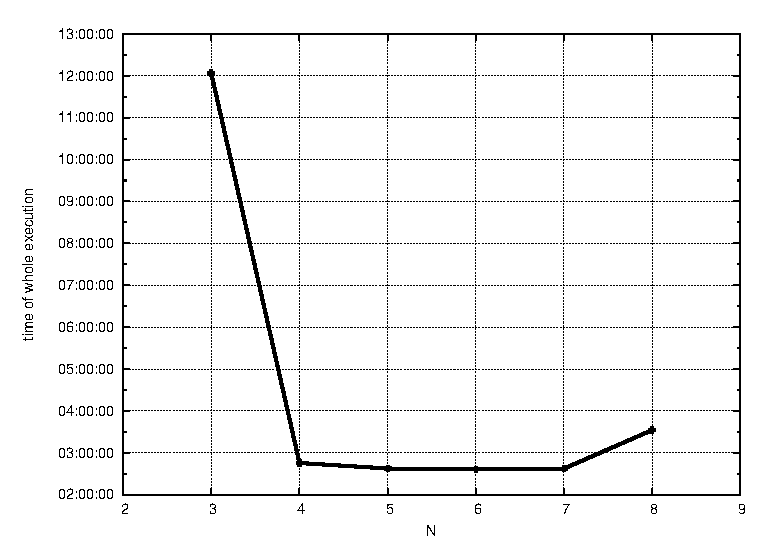
\includegraphics[width=\linewidth]{exp3-result.eps}
	\end{center}
	\caption{各$N$における実行時間}
	\label{pic:allN-time}
\end{figure}


図\ref{pic:time4all-process}に
$N=3, \ 6, \ 8$
における各ワーカーの全体実行時間(通信含む主要処理時間)を示す。
$N=6, \  8$では各ワーカーの全体実行時間がほぼすべて同じであるが、
$N=3$ではばらつきが出ている。
これは、$N=3$では問題が細かく分けられていなく、
マスタから受け取る陣によってワーカーの処理時間が異なることにより、
結果として各ワーカーの全体実行時間がつり合うように
仕事を分散できていないからだと考えられる。

また、図\ref{pic:time4all-only-correspondence}に
$N=3, \ 6, \ 8$
における各ワーカーの総通信時間(通信のみ)を示す。
$N=3, \ 6$では各ワーカーの総通信時間がほぼ0だが、
$N=8$では約50分ほどとなっている。
これは、$N=8$では問題が細かく分けられすぎていて、
マスタがワーカーに陣を配る回数が多くなり、
結果として通信をする際の
固定的処理時間が長くなってしまったからだと考えられる。

上記を考えると、
$N=6$の場合が、最も問題を分ける細かさと通信回数のバランスが取れており、
結果として最も実行時間が速くなったのだと考えられる。

\begin{figure}[htb]
	%\begin{minipage}{0.5\hsize}
		\begin{center}
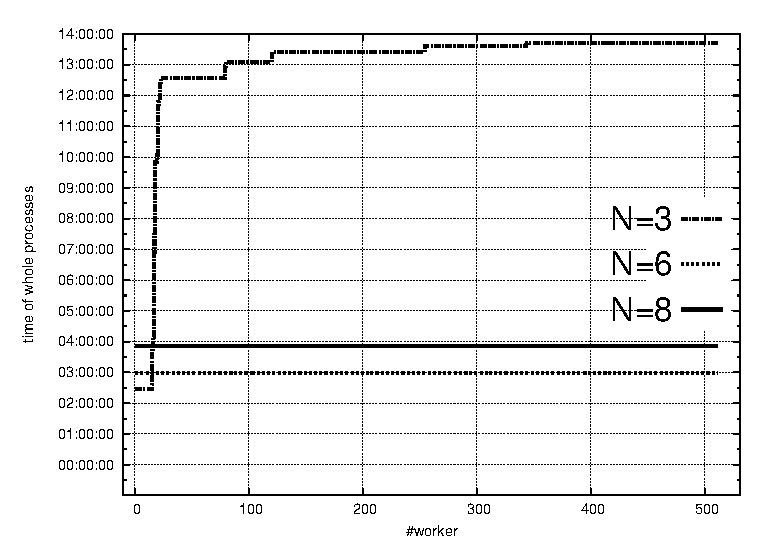
\includegraphics{exp4-2-tie.eps}
		\end{center}
		\caption{$N=3, \ 6, \ 8$における各ワーカーの全体実行時間}
		\label{pic:time4all-process}
	%\end{minipage}
\end{figure}
\begin{figure}[htb]
	%\begin{minipage}{0.5\hsize}
		\begin{center}
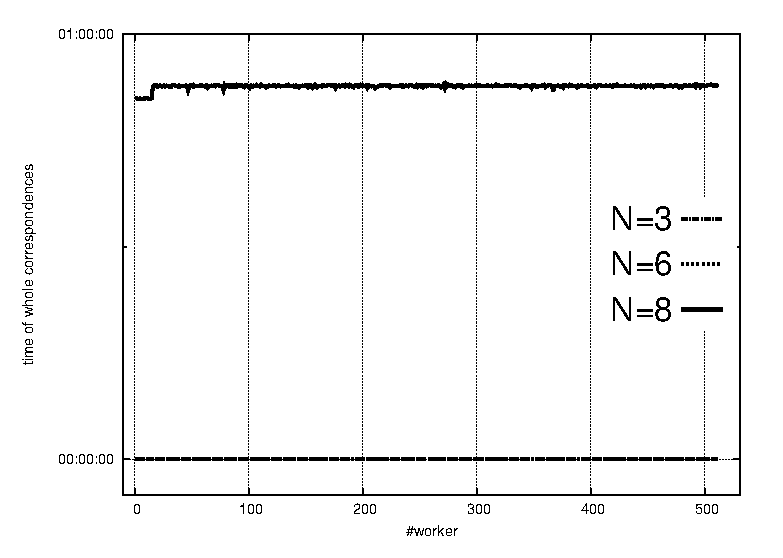
\includegraphics{exp4-2-tic.eps}
		\end{center}
		\caption{$N=3, \ 6, \ 8$における各ワーカーの総通信時間}
		\label{pic:time4all-only-correspondence}
	%\end{minipage}
\end{figure}
